\testfile{pgfplotstest.function.tex}
\testsection{`plot function' test}
\testsubsection{sin(x)}
\begin{tikzpicture}
\begin{axis}
\addplot plot[id=gnuplot_sin,samples=50] function{sin(x)};
\end{axis}
\end{tikzpicture}

\testsubsection{exp(x)}
\testsubsubsection{linear}
\begin{tikzpicture}
\begin{axis}
\addplot plot[id=gnuplot_exp,samples=50,domain=-5:15] function{exp(x)};
\end{axis}
\end{tikzpicture}

\testsubsubsection{semilogy}
\begin{tikzpicture}
\begin{semilogyaxis}
\addplot plot[id=gnuplot_exp,samples=50,domain=-5:15] function{exp(x)};
\end{semilogyaxis}
\end{tikzpicture}


\testsection{3D plots}
\testsubsection{plot expression}
{
	\pgfplotsset{samples=10,xlabel=x,ylabel=y}
	All plots use samples=10,/tikz/domain=0:360 as default!
	\tikzset{domain=0:360}

	\testsubsubsection{default params}
	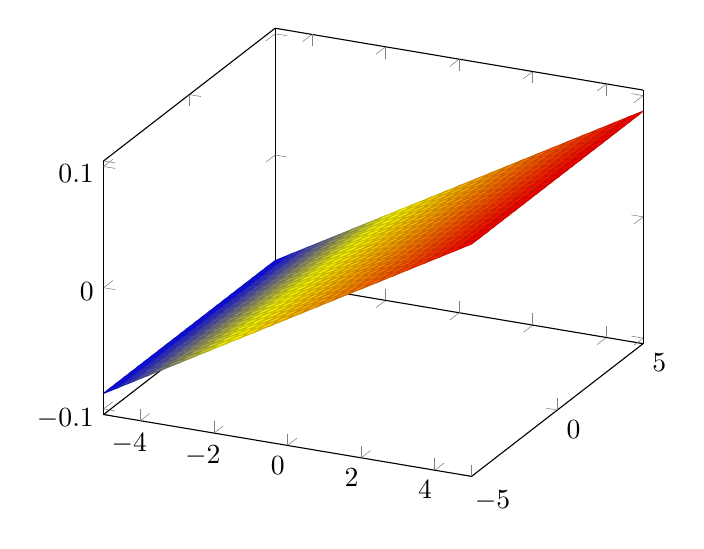
\begin{tikzpicture}
	\begin{axis}
	\addplot3[surf] {sin(x)};
	\end{axis}
	\end{tikzpicture}

	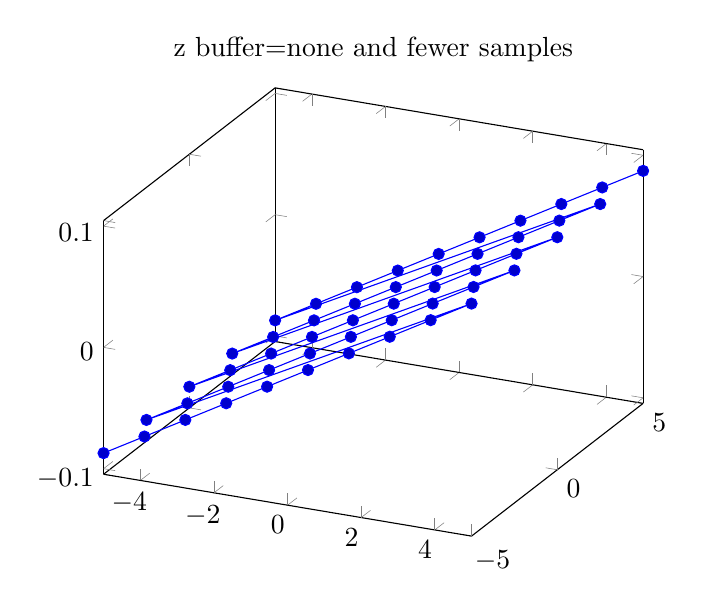
\begin{tikzpicture}
	\begin{axis}[z buffer=none,title={z buffer=none and fewer samples}]
	\addplot3+[samples=10,samples y=5] {sin(x)};
	\end{axis}
	\end{tikzpicture}

	\testsubsubsection{domain set}
	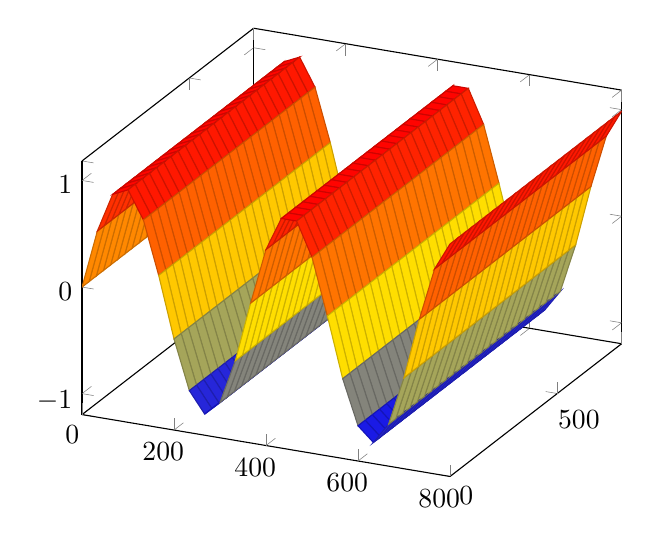
\begin{tikzpicture}
	\begin{axis}
	\addplot3[surf,domain=0:800] {sin(x)};
	\end{axis}
	\end{tikzpicture}

	\testsubsubsection{domain, domain y}
	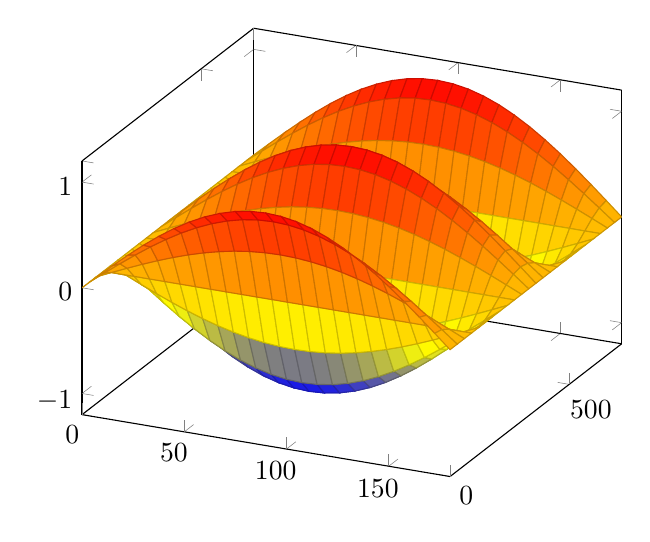
\begin{tikzpicture}
	\begin{axis}
	\addplot3[surf,domain=0:180,domain y=0:720] {sin(x) * cos(y)};
	\end{axis}
	\end{tikzpicture}

	\testsubsubsection{samples, samples y}
	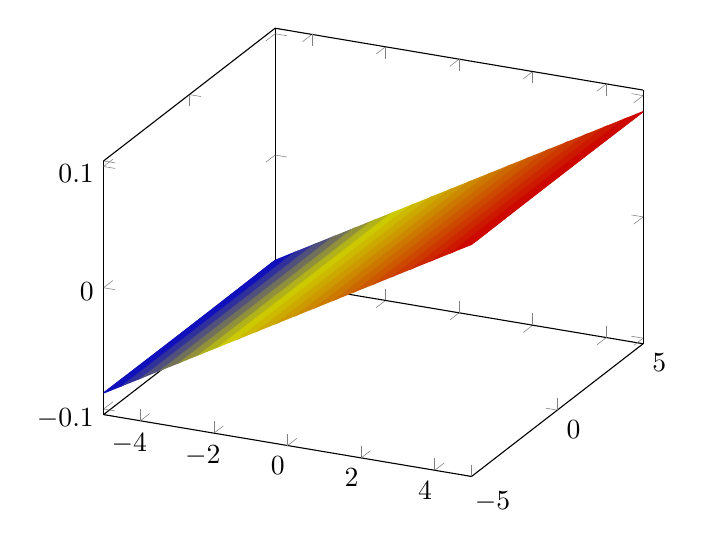
\begin{tikzpicture}
	\begin{axis}
	\addplot3[surf,samples=20,samples y=50] {sin(x) * cos(y)};
	\end{axis}
	\end{tikzpicture}

	\testsubsubsection{a line plot}
	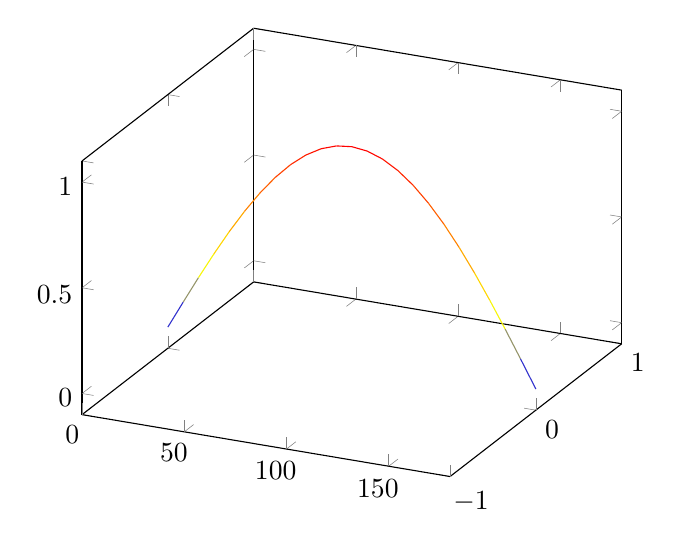
\begin{tikzpicture}
	\begin{axis}
	\addplot3[surf,domain=0:180,domain y=0:0] {sin(x)};
	\end{axis}
	\end{tikzpicture}

	\testsubsubsection{log in z (exp(x+y)}
		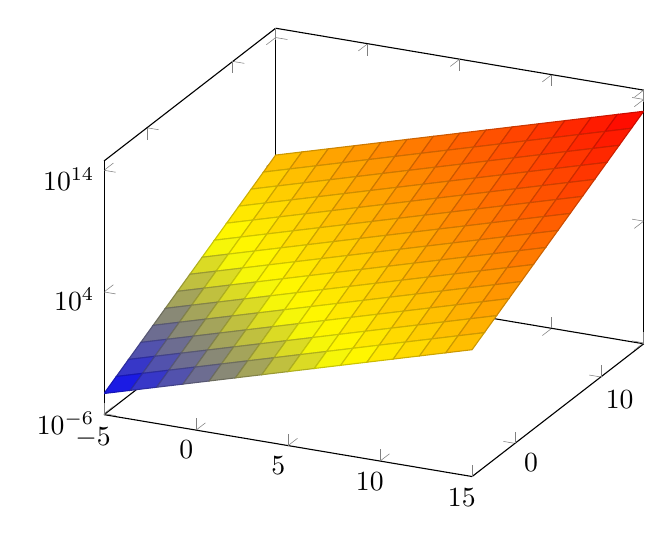
\begin{tikzpicture}
		\begin{axis}[zmode=log]
		\addplot3[surf,samples=15,domain=-5:15] {exp(x+y)};
		\end{axis}
		\end{tikzpicture}

}
\testsubsection{plot gnuplot}
{
	\pgfplotsset{samples=10,xlabel=x,ylabel=y}
	All plots use samples=10 as default!

	\testsubsubsection{default params}
	\begin{tikzpicture}
	\begin{axis}
	\addplot3[surf,id=3d_0] function{sin(x)};
	\end{axis}
	\end{tikzpicture}

	\begin{tikzpicture}
	\begin{axis}[z buffer=none,title={z buffer=none and fewer samples}]
	\addplot3+[id=3d_0,samples=10,samples y=5] function{sin(x)};
	\end{axis}
	\end{tikzpicture}

	\testsubsubsection{domain set}
	\begin{tikzpicture}
	\begin{axis}
	\addplot3[surf,id=3d_1,domain=0:7] function{sin(x)};
	\end{axis}
	\end{tikzpicture}

	\testsubsubsection{domain, domain y}
	\begin{tikzpicture}
	\begin{axis}
	\addplot3[surf,id=3d_2,domain=0:3,domain y=0:10] function{sin(x) * cos(y)};
	\end{axis}
	\end{tikzpicture}

	\testsubsubsection{samples, samples y}
	\begin{tikzpicture}
	\begin{axis}
	\addplot3[surf,id=3d_3,samples=20,samples y=50] function{sin(x) * cos(y)};
	\end{axis}
	\end{tikzpicture}
	%--------------------------------------------------
	% \begin{tikzpicture}
	% \begin{axis}[title={same with z buffer=sort}]
	% \addplot3[surf,id=3d_3,z buffer=sort,samples=20,samples y=50] function{sin(x) * cos(y)};
	% \end{axis}
	% \end{tikzpicture}
	%-------------------------------------------------- 

	%--------------------------------------------------
	%UNSUPPORTED BY GNUPLOT!?
	% \testsubsubsection{a line plot}
	% \begin{tikzpicture}
	% \begin{axis}
	% \addplot3[surf,id=3d_4,domain=0:3,domain y=0:0] function{sin(x)};
	% \end{axis}
	% \end{tikzpicture}
	%-------------------------------------------------- 

	\testsubsubsection{log in z (exp(x+y)}
		\begin{tikzpicture}
		\begin{axis}[zmode=log]
		\addplot3[surf,id=gnuplot_logz3d,samples=15,domain=-5:15] function{exp(x+y)};
		\end{axis}
		\end{tikzpicture}

\testsubsubsection{Checking the dummy variable names of the default config}
\begin{tikzpicture}
%\tracingmacros=2 \tracingcommands=2
	\begin{axis}
	\addplot gnuplot[id=gnuplot1d] {x};	
	\end{axis}
\end{tikzpicture}

\begin{tikzpicture}
	\begin{axis}
	\addplot3[mesh] gnuplot[id=gnuplot1d] {x + y};	
	\end{axis}
\end{tikzpicture}

\begin{tikzpicture}
	\begin{axis}
	\addplot gnuplot[id=gnuplot1dpar,parametric] {4*t^2,-t};	
	\end{axis}
\end{tikzpicture}

\begin{tikzpicture}
	\begin{axis}
	\addplot3[mesh] gnuplot[id=gnuplot2dpar,parametric] {u,v+u,v*u};	
	\end{axis}
\end{tikzpicture}

\testsubsubsection{non-standard values}
\begin{tikzpicture}
%\tracingmacros=2 \tracingcommands=2
	\begin{axis}
	\addplot gnuplot[id=gnuplot1d,variable=\h] {h};	
	\end{axis}
\end{tikzpicture}

\begin{tikzpicture}
%\tracingmacros=2 \tracingcommands=2
	\begin{axis}
	\addplot gnuplot[id=gnuplot1d,variable=h] {h};	
	\end{axis}
\end{tikzpicture}
}
